\chapter{Camins i circuits}

Aquest capítol parla de dos tipus de camins en els grafs:
\begin{itemize}
\item Un \key{Camí eulerià} és un camí que
travessa cada aresta exactament una vegada.
\item Un \key{Camí hamiltonià} és un camí
que visita cada node exactament una vegada.
\end{itemize}


Tot i que els camins eulerians i hamiltonians semblen conceptes
similars a primera vista, els problemes computacionals relacionats amb
ells són molt diferents. Resulta que hi ha una regla senzilla que
determina si un graf conté un camí eulerià, i també hi ha un algorisme
eficient per trobar aquest camí si existeix. Al contrari, comprovar
l'existència d'un camí hamiltonià és un problema NP-difícil, i no es
coneix cap algorisme eficient per resoldre el problema.

\section{Camins eulerians}

\index{Camí eulerià}

Una \key{camí eulerià}\footnote{L. Euler va estudiar aquests camins el
1736 quan va resoldre el famós problema del pont de Königsberg. Aquest
va ser el naixement de la teoria de grafs.} és un camí que passa
exactament una vegada per cada aresta del graf. Per exemple, el graf
\begin{center}
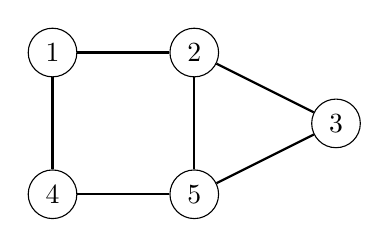
\begin{tikzpicture}[scale=0.9]
\node[draw, circle] (1) at (1,5) {$1$};
\node[draw, circle] (2) at (3,5) {$2$};
\node[draw, circle] (3) at (5,4) {$3$};
\node[draw, circle] (4) at (1,3) {$4$};
\node[draw, circle] (5) at (3,3) {$5$};

\path[draw,thick,-] (1) -- (2);
\path[draw,thick,-] (2) -- (3);
\path[draw,thick,-] (1) -- (4);
\path[draw,thick,-] (3) -- (5);
\path[draw,thick,-] (2) -- (5);
\path[draw,thick,-] (4) -- (5);
\end{tikzpicture}
\end{center}
té un camí eulerià des del node 2 fins al node 5:
\begin{center}
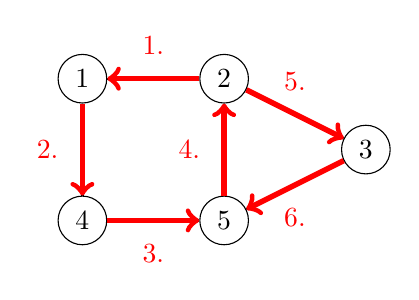
\begin{tikzpicture}[scale=0.9]
\node[draw, circle] (1) at (1,5) {$1$};
\node[draw, circle] (2) at (3,5) {$2$};
\node[draw, circle] (3) at (5,4) {$3$};
\node[draw, circle] (4) at (1,3) {$4$};
\node[draw, circle] (5) at (3,3) {$5$};

\path[draw,thick,-] (1) -- (2);
\path[draw,thick,-] (2) -- (3);
\path[draw,thick,-] (1) -- (4);
\path[draw,thick,-] (3) -- (5);
\path[draw,thick,-] (2) -- (5);
\path[draw,thick,-] (4) -- (5);

\path[draw=red,thick,->,line width=2pt] (2) -- node[font=\small,label={[red]north:1.}] {} (1);
\path[draw=red,thick,->,line width=2pt] (1) -- node[font=\small,label={[red]left:2.}] {} (4);
\path[draw=red,thick,->,line width=2pt] (4) -- node[font=\small,label={[red]south:3.}] {} (5);
\path[draw=red,thick,->,line width=2pt] (5) -- node[font=\small,label={[red]left:4.}] {} (2);
\path[draw=red,thick,->,line width=2pt] (2) -- node[font=\small,label={[red]north:5.}] {} (3);
\path[draw=red,thick,->,line width=2pt] (3) -- node[font=\small,label={[red]south:6.}] {} (5);
\end{tikzpicture}
\end{center}
\index{Circuit eulerià} Un \key{circuit eulerià} és un camí eulerià
que comença i acaba al mateix node. Per exemple, el graf
\begin{center}
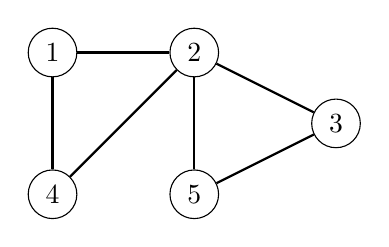
\begin{tikzpicture}[scale=0.9]
\node[draw, circle] (1) at (1,5) {$1$};
\node[draw, circle] (2) at (3,5) {$2$};
\node[draw, circle] (3) at (5,4) {$3$};
\node[draw, circle] (4) at (1,3) {$4$};
\node[draw, circle] (5) at (3,3) {$5$};

\path[draw,thick,-] (1) -- (2);
\path[draw,thick,-] (2) -- (3);
\path[draw,thick,-] (1) -- (4);
\path[draw,thick,-] (3) -- (5);
\path[draw,thick,-] (2) -- (5);
\path[draw,thick,-] (2) -- (4);
\end{tikzpicture}
\end{center}
té un circuit eulerià que comença i acaba al node 1:
\begin{center}
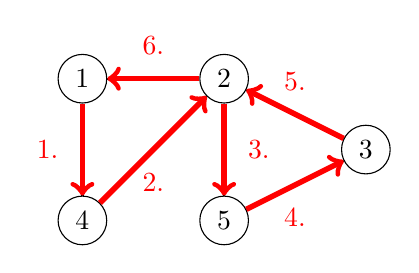
\begin{tikzpicture}[scale=0.9]
\node[draw, circle] (1) at (1,5) {$1$};
\node[draw, circle] (2) at (3,5) {$2$};
\node[draw, circle] (3) at (5,4) {$3$};
\node[draw, circle] (4) at (1,3) {$4$};
\node[draw, circle] (5) at (3,3) {$5$};

\path[draw,thick,-] (1) -- (2);
\path[draw,thick,-] (2) -- (3);
\path[draw,thick,-] (1) -- (4);
\path[draw,thick,-] (3) -- (5);
\path[draw,thick,-] (2) -- (5);
\path[draw,thick,-] (2) -- (4);

\path[draw=red,thick,->,line width=2pt] (1) -- node[font=\small,label={[red]left:1.}] {} (4);
\path[draw=red,thick,->,line width=2pt] (4) -- node[font=\small,label={[red]south:2.}] {} (2);
\path[draw=red,thick,->,line width=2pt] (2) -- node[font=\small,label={[red]right:3.}] {} (5);
\path[draw=red,thick,->,line width=2pt] (5) -- node[font=\small,label={[red]south:4.}] {} (3);
\path[draw=red,thick,->,line width=2pt] (3) -- node[font=\small,label={[red]north:5.}] {} (2);
\path[draw=red,thick,->,line width=2pt] (2) -- node[font=\small,label={[red]north:6.}] {} (1);
\end{tikzpicture}
\end{center}


\subsubsection{Existència}

L'existència de camins i circuits eulerians depèn dels graus dels
nodes. Un graf no dirigit té un camí eulerià exactament quan té un sol component
connex i
\begin{itemize}
\item el grau de cada node és parell \emph{o}
\item el grau de dos nodes és senar, i el grau de tots els altres nodes és parell.
\end{itemize}


En el primer cas, cada camí eulerià és també un circuit eulerià. En el
segon cas, els nodes de grau senar són els nodes inicials i finals
d'un camí eulerià que no és un circuit eulerià \footnote{(N. del T.)
És clar que, si un graf té un node de grau senar, no pot tenir un
circuit eulerià, perquè els circuits eulerians tenen tots els nodes de
grau parell. Allò sorprenent és que aquesta condició també sigui
suficient.}.

Per exemple, en el graf  
\begin{center}
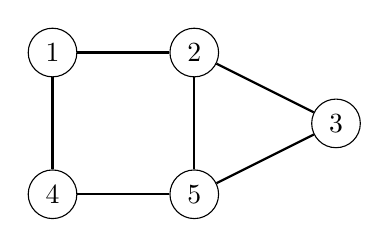
\begin{tikzpicture}[scale=0.9]
\node[draw, circle] (1) at (1,5) {$1$};
\node[draw, circle] (2) at (3,5) {$2$};
\node[draw, circle] (3) at (5,4) {$3$};
\node[draw, circle] (4) at (1,3) {$4$};
\node[draw, circle] (5) at (3,3) {$5$};

\path[draw,thick,-] (1) -- (2);
\path[draw,thick,-] (2) -- (3);
\path[draw,thick,-] (1) -- (4);
\path[draw,thick,-] (3) -- (5);
\path[draw,thick,-] (2) -- (5);
\path[draw,thick,-] (4) -- (5);
\end{tikzpicture}
\end{center}

els nodes 1, 3 i 4 tenen grau 2, i els nodes 2 i 5 tenen grau
3. Com que hi ha dos nodes de grau senar, hi ha un camí eulerià entre
els nodes 2 i 5, però el graf no conté cap circuit eulerià.

En un graf dirigit ens fixem en els graus d'entrada i sortida dels
nodes. Un graf dirigit conté un camí eulerià exactament quan té un sol
component connex i
\begin{itemize}
\item en tots els nodes el grau d'entrada és igual al grau de sortida, \emph{o}
\item hi ha un node on el grau d'entrada és un més que el grau de sortida,
  hi ha un altre node on el grau de sortida és un més que el grau d'entrada,
  i en tots els altres nodes el grau d'entrada és igual al grau de sortida.
\end{itemize}

En el primer cas, cada camí eulerià també és un circuit eulerià, i en
el segon cas, el graf conté un camí eulerià que comença al node amb excés
de grau de sortida i acaba al node amb excés de grau d'entrada.

Per exemple, al graf
\begin{center}
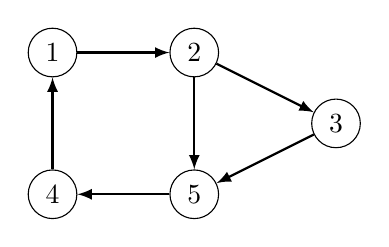
\begin{tikzpicture}[scale=0.9]
\node[draw, circle] (1) at (1,5) {$1$};
\node[draw, circle] (2) at (3,5) {$2$};
\node[draw, circle] (3) at (5,4) {$3$};
\node[draw, circle] (4) at (1,3) {$4$};
\node[draw, circle] (5) at (3,3) {$5$};

\path[draw,thick,->,>=latex] (1) -- (2);
\path[draw,thick,->,>=latex] (2) -- (3);
\path[draw,thick,->,>=latex] (4) -- (1);
\path[draw,thick,->,>=latex] (3) -- (5);
\path[draw,thick,->,>=latex] (2) -- (5);
\path[draw,thick,->,>=latex] (5) -- (4);
\end{tikzpicture}
\end{center}
els nodes 1, 3 i 4 tenen grau d'entrada i de sortida 1, el node 2 té grau d'entrada 1 i grau de sortida 2, i el node 5 té grau d'entrada 2 i grau de sortida 1. Per tant,
el graf conté un camí eulerià des del node 2 fins al node 5:
\begin{center}
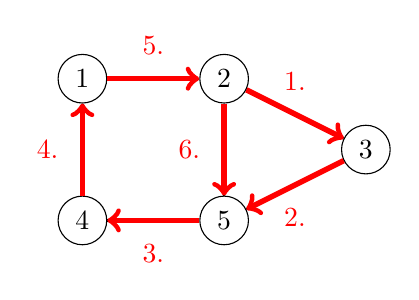
\begin{tikzpicture}[scale=0.9]
\node[draw, circle] (1) at (1,5) {$1$};
\node[draw, circle] (2) at (3,5) {$2$};
\node[draw, circle] (3) at (5,4) {$3$};
\node[draw, circle] (4) at (1,3) {$4$};
\node[draw, circle] (5) at (3,3) {$5$};

\path[draw,thick,-] (1) -- (2);
\path[draw,thick,-] (2) -- (3);
\path[draw,thick,-] (1) -- (4);
\path[draw,thick,-] (3) -- (5);
\path[draw,thick,-] (2) -- (5);
\path[draw,thick,-] (4) -- (5);

\path[draw=red,thick,->,line width=2pt] (2) -- node[font=\small,label={[red]north:1.}] {} (3);
\path[draw=red,thick,->,line width=2pt] (3) -- node[font=\small,label={[red]south:2.}] {} (5);
\path[draw=red,thick,->,line width=2pt] (5) -- node[font=\small,label={[red]south:3.}] {} (4);
\path[draw=red,thick,->,line width=2pt] (4) -- node[font=\small,label={[red]left:4.}] {} (1);
\path[draw=red,thick,->,line width=2pt] (1) -- node[font=\small,label={[red]north:5.}] {} (2);
\path[draw=red,thick,->,line width=2pt] (2) -- node[font=\small,label={[red]left:6.}] {} (5);
\end{tikzpicture}
\end{center}


\subsubsection{Algorisme de Hierholzer}

\index{Algorisme de Hierholzer}

\key{Algorisme de Hierholzer}\footnote{L'algorisme es va publicar el
1873 després de la mort de Hierholzer \cite{hie73}.} és un mètode
eficient per construir un circuit eulerià. L'algorisme consta de
diverses rondes, cadascuna de les quals afegeix noves arestes al
circuit. Suposem que el graf conté un circuit eulerià; en cas contrari
l'algorisme de Hierholzer no el pot trobar.

En primer lloc, l'algorisme construeix un circuit que conté algunes
(no necessàriament totes) les arestes del graf. Després d'això,
l'algorisme amplia el circuit pas a pas afegint-hi subcircuits. El
procés continua fins que totes les arestes s'han afegit al circuit.

L'algorisme sempre amplia el circuit mitjançant un node $x$ que
pertany al circuit però que té una aresta de sortida que no pertany al
circuit.  L'algorisme construeix un nou camí des del node $x$ només
amb arestes que no pertanyen al circuit. Tard o d'hora, el camí
tornarà al node $x$, creant un nou subcircuit que afegim al circuit
original.

Si el graf només conté camins eulerians, també podem trobar-los amb
l'algorisme de Hierholzer, afegint una aresta addicional al graf entre
els dos nodes especials i eliminant-la després de construir el
circuit. Per exemple, en un graf no dirigit, afegim l'aresta
addicional entre els dos nodes de grau senar.

A continuació veurem com l'algorisme de Hierholzer construeix un
circuit eulerià per a un graf no dirigit.

\subsubsection{Exemple}


\begin{samepage}
Considerem el graf següent:
\begin{center}
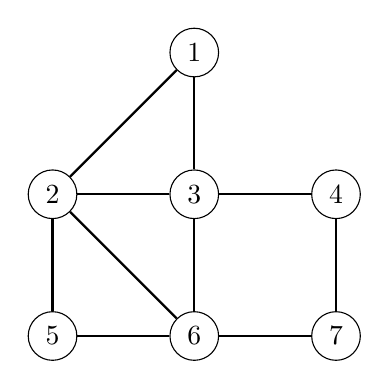
\begin{tikzpicture}[scale=0.9]
\node[draw, circle] (1) at (3,5) {$1$};
\node[draw, circle] (2) at (1,3) {$2$};
\node[draw, circle] (3) at (3,3) {$3$};
\node[draw, circle] (4) at (5,3) {$4$};
\node[draw, circle] (5) at (1,1) {$5$};
\node[draw, circle] (6) at (3,1) {$6$};
\node[draw, circle] (7) at (5,1) {$7$};

\path[draw,thick,-] (1) -- (2);
\path[draw,thick,-] (1) -- (3);
\path[draw,thick,-] (2) -- (3);
\path[draw,thick,-] (2) -- (5);
\path[draw,thick,-] (2) -- (6);
\path[draw,thick,-] (3) -- (4);
\path[draw,thick,-] (3) -- (6);
\path[draw,thick,-] (4) -- (7);
\path[draw,thick,-] (5) -- (6);
\path[draw,thick,-] (6) -- (7);
\end{tikzpicture}
\end{center}
\end{samepage}


\begin{samepage}
Suposem que l'algorisme primer crea un circuit que comença al node 1. Un
circuit possible és
$1 \rightarrow 2 \rightarrow 3 \rightarrow 1$:
\begin{center}
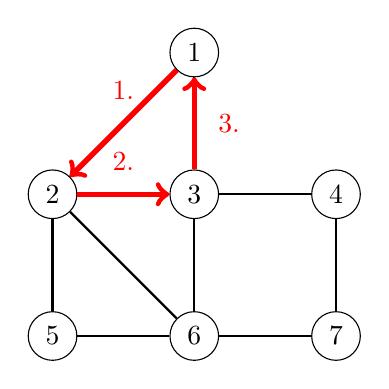
\begin{tikzpicture}[scale=0.9]
\node[draw, circle] (1) at (3,5) {$1$};
\node[draw, circle] (2) at (1,3) {$2$};
\node[draw, circle] (3) at (3,3) {$3$};
\node[draw, circle] (4) at (5,3) {$4$};
\node[draw, circle] (5) at (1,1) {$5$};
\node[draw, circle] (6) at (3,1) {$6$};
\node[draw, circle] (7) at (5,1) {$7$};

\path[draw,thick,-] (1) -- (2);
\path[draw,thick,-] (1) -- (3);
\path[draw,thick,-] (2) -- (3);
\path[draw,thick,-] (2) -- (5);
\path[draw,thick,-] (2) -- (6);
\path[draw,thick,-] (3) -- (4);
\path[draw,thick,-] (3) -- (6);
\path[draw,thick,-] (4) -- (7);
\path[draw,thick,-] (5) -- (6);
\path[draw,thick,-] (6) -- (7);

\path[draw=red,thick,->,line width=2pt] (1) -- node[font=\small,label={[red]north:1.}] {} (2);
\path[draw=red,thick,->,line width=2pt] (2) -- node[font=\small,label={[red]north:2.}] {} (3);
\path[draw=red,thick,->,line width=2pt] (3) -- node[font=\small,label={[red]east:3.}] {} (1);
\end{tikzpicture}
\end{center}
\end{samepage}
Després d'això, l'algorisme afegeix el subcircuit $2 \rightarrow 5
\rightarrow 6 \rightarrow 2$ al circuit:
\begin{center}
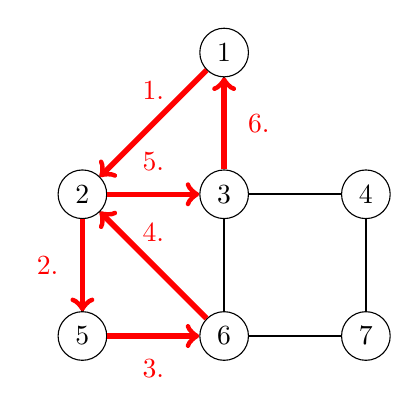
\begin{tikzpicture}[scale=0.9]
\node[draw, circle] (1) at (3,5) {$1$};
\node[draw, circle] (2) at (1,3) {$2$};
\node[draw, circle] (3) at (3,3) {$3$};
\node[draw, circle] (4) at (5,3) {$4$};
\node[draw, circle] (5) at (1,1) {$5$};
\node[draw, circle] (6) at (3,1) {$6$};
\node[draw, circle] (7) at (5,1) {$7$};

\path[draw,thick,-] (1) -- (2);
\path[draw,thick,-] (1) -- (3);
\path[draw,thick,-] (2) -- (3);
\path[draw,thick,-] (2) -- (5);
\path[draw,thick,-] (2) -- (6);
\path[draw,thick,-] (3) -- (4);
\path[draw,thick,-] (3) -- (6);
\path[draw,thick,-] (4) -- (7);
\path[draw,thick,-] (5) -- (6);
\path[draw,thick,-] (6) -- (7);

\path[draw=red,thick,->,line width=2pt] (1) -- node[font=\small,label={[red]north:1.}] {} (2);
\path[draw=red,thick,->,line width=2pt] (2) -- node[font=\small,label={[red]west:2.}] {} (5);
\path[draw=red,thick,->,line width=2pt] (5) -- node[font=\small,label={[red]south:3.}] {} (6);
\path[draw=red,thick,->,line width=2pt] (6) -- node[font=\small,label={[red]north:4.}] {} (2);
\path[draw=red,thick,->,line width=2pt] (2) -- node[font=\small,label={[red]north:5.}] {} (3);
\path[draw=red,thick,->,line width=2pt] (3) -- node[font=\small,label={[red]east:6.}] {} (1);
\end{tikzpicture}
\end{center}
Finalment, l'algorisme afegeix el subcircuit $6 \rightarrow 3
\rightarrow 4 \rightarrow 7 \rightarrow 6$ al circuit:
\begin{center}
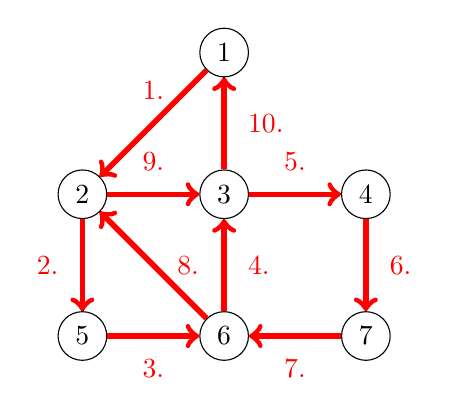
\begin{tikzpicture}[scale=0.9]
\node[draw, circle] (1) at (3,5) {$1$};
\node[draw, circle] (2) at (1,3) {$2$};
\node[draw, circle] (3) at (3,3) {$3$};
\node[draw, circle] (4) at (5,3) {$4$};
\node[draw, circle] (5) at (1,1) {$5$};
\node[draw, circle] (6) at (3,1) {$6$};
\node[draw, circle] (7) at (5,1) {$7$};

\path[draw,thick,-] (1) -- (2);
\path[draw,thick,-] (1) -- (3);
\path[draw,thick,-] (2) -- (3);
\path[draw,thick,-] (2) -- (5);
\path[draw,thick,-] (2) -- (6);
\path[draw,thick,-] (3) -- (4);
\path[draw,thick,-] (3) -- (6);
\path[draw,thick,-] (4) -- (7);
\path[draw,thick,-] (5) -- (6);
\path[draw,thick,-] (6) -- (7);

\path[draw=red,thick,->,line width=2pt] (1) -- node[font=\small,label={[red]north:1.}] {} (2);
\path[draw=red,thick,->,line width=2pt] (2) -- node[font=\small,label={[red]west:2.}] {} (5);
\path[draw=red,thick,->,line width=2pt] (5) -- node[font=\small,label={[red]south:3.}] {} (6);
\path[draw=red,thick,->,line width=2pt] (6) -- node[font=\small,label={[red]east:4.}] {} (3);
\path[draw=red,thick,->,line width=2pt] (3) -- node[font=\small,label={[red]north:5.}] {} (4);
\path[draw=red,thick,->,line width=2pt] (4) -- node[font=\small,label={[red]east:6.}] {} (7);
\path[draw=red,thick,->,line width=2pt] (7) -- node[font=\small,label={[red]south:7.}] {} (6);
\path[draw=red,thick,->,line width=2pt] (6) -- node[font=\small,label={[red]right:8.}] {} (2);
\path[draw=red,thick,->,line width=2pt] (2) -- node[font=\small,label={[red]north:9.}] {} (3);
\path[draw=red,thick,->,line width=2pt] (3) -- node[font=\small,label={[red]east:10.}] {} (1);
\end{tikzpicture}
\end{center}
Ara totes les arestes estan incloses al circuit, així que hem
construït amb èxit un circuit eulerià.

\section{Camins de Hamilton}

\index{Camí de Hamilton}

Un \key{camí hamiltonià} %\footnote{W. R. Hamilton (1805--1865) va ser un matemàtic irlandès.}
és un camí que visita cada node del graf exactament una vegada. Per exemple, el graf
\begin{center}
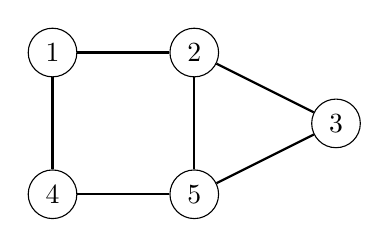
\begin{tikzpicture}[scale=0.9]
\node[draw, circle] (1) at (1,5) {$1$};
\node[draw, circle] (2) at (3,5) {$2$};
\node[draw, circle] (3) at (5,4) {$3$};
\node[draw, circle] (4) at (1,3) {$4$};
\node[draw, circle] (5) at (3,3) {$5$};

\path[draw,thick,-] (1) -- (2);
\path[draw,thick,-] (2) -- (3);
\path[draw,thick,-] (1) -- (4);
\path[draw,thick,-] (3) -- (5);
\path[draw,thick,-] (2) -- (5);
\path[draw,thick,-] (4) -- (5);
\end{tikzpicture}
\end{center}
conté un camí hamiltonià des del node 1 fins al node 3:
\begin{center}
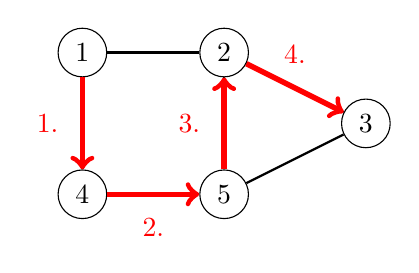
\begin{tikzpicture}[scale=0.9]
\node[draw, circle] (1) at (1,5) {$1$};
\node[draw, circle] (2) at (3,5) {$2$};
\node[draw, circle] (3) at (5,4) {$3$};
\node[draw, circle] (4) at (1,3) {$4$};
\node[draw, circle] (5) at (3,3) {$5$};

\path[draw,thick,-] (1) -- (2);
\path[draw,thick,-] (2) -- (3);
\path[draw,thick,-] (1) -- (4);
\path[draw,thick,-] (3) -- (5);
\path[draw,thick,-] (2) -- (5);
\path[draw,thick,-] (4) -- (5);

\path[draw=red,thick,->,line width=2pt] (1) -- node[font=\small,label={[red]left:1.}] {} (4);
\path[draw=red,thick,->,line width=2pt] (4) -- node[font=\small,label={[red]south:2.}] {} (5);
\path[draw=red,thick,->,line width=2pt] (5) -- node[font=\small,label={[red]left:3.}] {} (2);
\path[draw=red,thick,->,line width=2pt] (2) -- node[font=\small,label={[red]north:4.}] {} (3);
\end{tikzpicture}
\end{center}


\index{Circuit Hamiltonià}

Si un camí hamiltonià comença i acaba al mateix node, s'anomena
\key{circuit hamiltonià}. El graf anterior també té un circuit
hamiltonià que comença i acaba al node 1:
\begin{center}
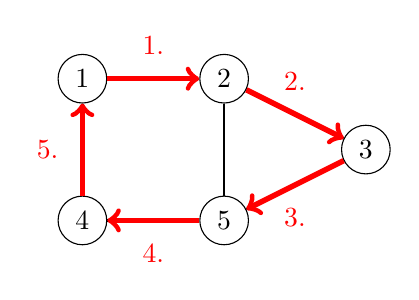
\begin{tikzpicture}[scale=0.9]
\node[draw, circle] (1) at (1,5) {$1$};
\node[draw, circle] (2) at (3,5) {$2$};
\node[draw, circle] (3) at (5,4) {$3$};
\node[draw, circle] (4) at (1,3) {$4$};
\node[draw, circle] (5) at (3,3) {$5$};

\path[draw,thick,-] (1) -- (2);
\path[draw,thick,-] (2) -- (3);
\path[draw,thick,-] (1) -- (4);
\path[draw,thick,-] (3) -- (5);
\path[draw,thick,-] (2) -- (5);
\path[draw,thick,-] (4) -- (5);

\path[draw=red,thick,->,line width=2pt] (1) -- node[font=\small,label={[red]north:1.}] {} (2);
\path[draw=red,thick,->,line width=2pt] (2) -- node[font=\small,label={[red]north:2.}] {} (3);
\path[draw=red,thick,->,line width=2pt] (3) -- node[font=\small,label={[red]south:3.}] {} (5);
\path[draw=red,thick,->,line width=2pt] (5) -- node[font=\small,label={[red]south:4.}] {} (4);
\path[draw=red,thick,->,line width=2pt] (4) -- node[font=\small,label={[red]left:5.}] {} (1);
\end{tikzpicture}
\end{center}


\subsubsection{Existència}

No es coneix cap mètode eficient per provar si un graf conté un camí
hamiltonià, i el problema és NP-difícil. Tot i així, en alguns casos
especials, podem estar segurs que un graf conté un camí hamiltonià.

Una observació senzilla és que si el graf és complet, és a dir, si hi
ha una aresta entre tots els parells de nodes, aleshores també conté
un camí hamiltonià. També hi ha resultats més forts:

\begin{itemize}
\item
\index{Teorema de Dirac}
\key{Teorema de Dirac}: %\cite{dir52}
Si el grau de cada node és almenys $n/2$,
el graf conté un camí hamiltonià.
\item
\index{Teorema d'Ore}
\key{Teorema d'Ore}: %\cite{ore60}
Si la suma de graus de cada parell de nodes no adjacents
és almenys $n$,
el graf conté un camí hamiltonià.
\end{itemize}


Una propietat comuna en aquests teoremes i altres resultats és que
garanteixen l'existència d'un camí hamiltonià si el graf té \emph{un
gran nombre} d'arestes. Això té sentit, perquè com més arestes conté
el graf, més possibilitats hi ha de construir un camí hamiltonià.

\subsubsection{Construcció}

Com que no hi ha cap manera eficient de comprovar si existeix un camí
hamiltonià, és clar que tampoc no hi ha cap mètode per construir el
camí de manera eficient, perquè en cas contrari simplement intentaríem
construir el camí i miraríem si tenim èxit.

Una manera senzilla de buscar un camí hamiltonià és amb un algorisme
de marxa enrera (\emph{backtracking}) que passi per totes les maneres
possibles de construir el camí. La complexitat temporal d'aquest
algorisme és com a molt $O(n!)$, perquè hi ha $n!$ maneres diferents
d'ordenar $n$ nodes.

Una solució més eficient fa servir programació dinàmica (vegeu el
capítol~\ref{bits-dp}). La idea és calcular els valors d'una funció
$\texttt{possible}(S,x)$, on $S$ és un subconjunt de nodes i $x$ és un
dels nodes. La funció indica si hi ha un camí hamiltonià que visita
els nodes de $S$ i acaba al node $x$. És possible implementar aquesta
solució en temps $O(2^n n^2)$.

\section{Seqüències de De Bruijn}

\index{Seqüència de De Bruijn}

Una \key{seqüència de De Bruijn} és una cadena que conté cada subcadena
de longitud $n$ exactament una vegada com a subcadena, per a un
alfabet fix de $k$ caràcters. La longitud d'aquesta cadena és de
$k^n+n-1$ caràcters. Per exemple, quan $n=3$ i $k=2$, un exemple de
seqüència de De Bruijn és
\[0001011100.\]
Les subcadenes d'aquesta cadena són totes les combinacions de tres bits:
000, 001, 010, 011, 100, 101, 110 i 111.

Resulta que cada seqüència de De Bruijn es correspon amb un camí eulerià en
un graf. La idea és construir un graf on cada node contingui una
cadena de $n-1$ caràcters i cada aresta afegeix un caràcter a la
cadena. El graf següent correspon a l'escenari anterior:


\begin{center}
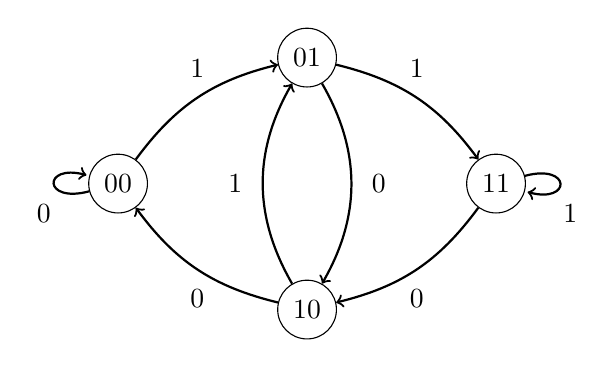
\begin{tikzpicture}[scale=0.8]
\node[draw, circle] (00) at (-3,0) {00};
\node[draw, circle] (11) at (3,0) {11};
\node[draw, circle] (01) at (0,2) {01};
\node[draw, circle] (10) at (0,-2) {10};

\path[draw,thick,->] (00) edge [bend left=20] node[font=\small,label=1] {} (01);
\path[draw,thick,->] (01) edge [bend left=20] node[font=\small,label=1] {} (11);
\path[draw,thick,->] (11) edge [bend left=20] node[font=\small,label=below:0] {} (10);
\path[draw,thick,->] (10) edge [bend left=20] node[font=\small,label=below:0] {} (00);

\path[draw,thick,->] (01) edge [bend left=30] node[font=\small,label=right:0] {} (10);
\path[draw,thick,->] (10) edge [bend left=30] node[font=\small,label=left:1] {} (01);

\path[draw,thick,-] (00) edge [loop left] node[font=\small,label=below:0] {} (00);
\path[draw,thick,-] (11) edge [loop right] node[font=\small,label=below:1] {} (11);
\end{tikzpicture}
\end{center}


Un camí eulerià en aquest graf correspon a una cadena que conté totes
les cadenes de longitud $n$. La cadena conté els caràcters del node
inicial i tots els caràcters de les arestes. El node inicial té $n-1$
caràcters i hi ha $k^n$ caràcters a les arestes, de manera que la
longitud de la cadena és $k^n+n-1$.

\section{Ruta del cavall}

\index{ruta del cavall}

Una \key{ruta del cavall} és una seqüència de moviments d'un cavall en
un tauler d'escacs $n \times n$, seguint les regles dels escacs, de
manera que el cavall visita cada casella exactament una vegada. La
ruta del cavall és \emph{tancada} si el cavall torna a la casella
inicial i, en cas contrari, és \emph{oberta}.

Per exemple, aquí hi ha una ruta oberta del cavall en un tauler de $5 \times 5$:


\begin{center}
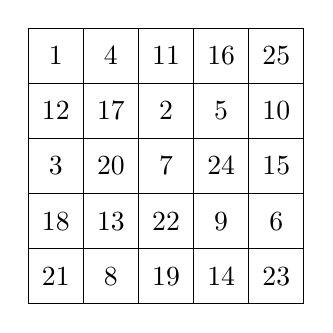
\begin{tikzpicture}[scale=0.7]
\draw (0,0) grid (5,5);
\node at (0.5,4.5) {$1$};
\node at (1.5,4.5) {$4$};
\node at (2.5,4.5) {$11$};
\node at (3.5,4.5) {$16$};
\node at (4.5,4.5) {$25$};
\node at (0.5,3.5) {$12$};
\node at (1.5,3.5) {$17$};
\node at (2.5,3.5) {$2$};
\node at (3.5,3.5) {$5$};
\node at (4.5,3.5) {$10$};
\node at (0.5,2.5) {$3$};
\node at (1.5,2.5) {$20$};
\node at (2.5,2.5) {$7$};
\node at (3.5,2.5) {$24$};
\node at (4.5,2.5) {$15$};
\node at (0.5,1.5) {$18$};
\node at (1.5,1.5) {$13$};
\node at (2.5,1.5) {$22$};
\node at (3.5,1.5) {$9$};
\node at (4.5,1.5) {$6$};
\node at (0.5,0.5) {$21$};
\node at (1.5,0.5) {$8$};
\node at (2.5,0.5) {$19$};
\node at (3.5,0.5) {$14$};
\node at (4.5,0.5) {$23$};
\end{tikzpicture}
\end{center}


Una ruta del cavall es correspon a un camí hamiltonià en un graf els
nodes del qual representen les caselles del tauler, i dos nodes estan
connectats amb una aresta si un cavall pot moure's entre elles segons
les regles dels escacs.

Una manera natural de construir una ruta del cavall és amb
\emph{backtracking}. La cerca es pot fer més eficient fent servir
\emph{heurístiques} que intenten guiar el cavall de manera que
trobi ràpidament una ruta sencera.

\subsubsection{Regla de Warnsdorf}

\index{heurística} \index{Regla de Warnsdorf}

\key{La regla de Warnsdorf} és una heurística senzilla i eficaç per
trobar una ruta del cavall\footnote{Aquesta heurística es va proposar
al llibre de Warnsdorf \cite{war23} l'any 1823. També hi ha algorismes
polinomials per trobar les rutes del cavall \cite{par97}, però són més
complicats.}. Utilitzant la regla, és possible construir de manera
eficient una ruta fins i tot en un tauler gran. La idea és moure el
cavall a una casella on el nombre de moviments possibles sigui el més
\emph{petit} possible.

Per exemple, en la situació següent, hi ha cinc caselles possibles a
les quals es pot moure el cavall (quadrats $a \ldots e$):
\begin{center}
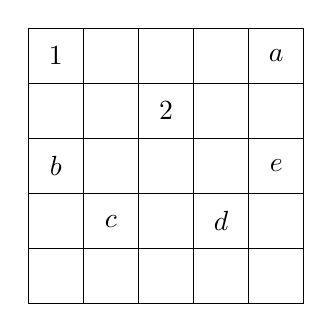
\begin{tikzpicture}[scale=0.7]
\draw (0,0) grid (5,5);
\node at (0.5,4.5) {$1$};
\node at (2.5,3.5) {$2$};
\node at (4.5,4.5) {$a$};
\node at (0.5,2.5) {$b$};
\node at (4.5,2.5) {$e$};
\node at (1.5,1.5) {$c$};
\node at (3.5,1.5) {$d$};
\end{tikzpicture}
\end{center}
En aquesta situació, la regla de Warnsdorf mou el cavall al quadrat
$a$, perquè després d'aquesta elecció només hi ha un únic moviment
possible, mentre que les altres opcions mouen el cavall a caselles on
hi ha tres moviments possibles.
